% Include required packages
\documentclass{mxl-design}
\usepackage{listings}
\usepackage{float}
\usepackage{enumitem}

%====== Title Page ======%
% Setup document
\title{Mercury2 Revised Design}
\author{Jimmy Blanchard}
\docnum{0.3.0}
\setcounter{secnumdepth}{4}

% Start the document
\begin{document}
\maketitle

% Document revision history
\vspace{5in}
\begin{table}[H]
\begin{center}
\begin{tabular}{|p{0.5in}|p{1.2in}|p{2.8in}|p{0.5in}|}
	\hline
	\bf Rev & \bf Date & \bf Notes & \bf Authors \\ 
	\hline
	0.3.0 & December 2, 2012 & Mercury2 design revisions. & jimblanc \\ \hline
\end{tabular}
\end{center}
\end{table}

%====== Table of Contents ======%
\clearpage
\tableofcontents
\clearpage

%==========================%
%====== Introduction ======%
%==========================%
\part{Introduction}
Mercury2 is the next evolution of the Mercury Ground Station System. It will allow satellite operators to reserve, configure, and use ground station hardware while still giving ground station operators complete control over their hardware. Mercury2 will include a feature rich web interface to enable ground station control over the network by satellite and ground station operators alike.

%=== Terms ===%
\section{Terms and Definitions}
\label{sec:terms}
This section contains a list terms and acronyms commonly used in this document.

\begin{table}[h]
	\footnotesize {\begin{tabular}{ p{5cm} p{10cm} }
		\textbf{Mercury2} & Refers to the ground station management system as a whole, including all sub-components (e.g. the hardware manager and user interface).\\[.2cm]
		\textbf{Hardware Manager} & An application that runs on a computer that is physically attached to the ground station hardware. It is responsible for processing ground station commands (from the user interface) and facilitating data transfer.\\[.2cm]
		\textbf{User Interface} & This application runs on a web server and provides the interfaces to allow ground station and satellite operators to interact with and control the ground station. It relays commands from the user to the hardware manager.\\[.2cm]
		\textbf{Hardware Pipeline} & A collection of related hardware used to either transmit or receive information to and from the radio (or both, if the hardware supports it).\\[.2cm]
		\textbf{Ground Station} & Refers to the complete Mercury2 system (i.e. the user interface and any hardware managers associated with it). Generally, this means several computers and pieces of hardware on the same local area network.\\[.2cm]
		\textbf{Satellite} & A device in orbit that Mercury2 configured ground stations can connect to.\\[.2cm]
		\textbf{Pass} & A transit of a satellite over a ground station. Passes can be scheduled, which reserves a specific hardware pipeline for the duration of the pass. Scheduled passes are identified by the satellite name, orbit number, and ground station.\\[.2cm]
		\textbf{Timestamp} & The duration of scheduled command sessions for Mercury2 will be defined by a start and end timestamp. These timestamps will be simple UNIX timestamps indicating the start and end of the reservation.\\[.2cm]
		\textbf{Satellite Operator} & An entity that remotely reserves ground station use (via the user interface) and uses it to send and receive data from a satellite.\\[.2cm]
		\textbf{Ground Station Operator} & A user that is associated with the ground station and has some privileges over it (e.g. the ability to approve/reject reservation requests or the ability to configure hardware pipelines).\\[.2cm]
		\textbf{Ground Station Administrator} & The user with complete administrative control over the ground station.\\[.2cm]
		\textbf{MVC Framework} & Model-View-Controller framework. Refers to a common web application software design pattern.\\[.2cm]
		\textbf{YAML} & An easy-to-use configuration format. Will be used to configure the hardware manager.\\[.2cm]
		\textbf{Asynchronous} & A type of program design that allows tasks to be executed in an undefined order. This will be used in the hardware manager to allow it to respond to radio events.
	\end{tabular}}
	\caption{General Definitions}
	\label{tab:Mercury2 Definitions}
\end{table}

%=== Requirements ===%
\clearpage
\section{Application Requirements}
This section outlines the various requirements for the Mercury2 system. These are the requirements for the initial release of the application.

\subsection{User Interface Requirements}
The user interface component of Mercury2 will run on a net-accessible web server and will allow satellite and ground station operators to interact with the various configured hardware managers. Its primary features consist of the following items.

\begin{itemize}
	\item User authentication, authorization, and management
		\begin{itemize}
			\item Registration and account management
			\item API access key management
			\item User permissions
		\end{itemize}
	\item Ground station administration
		\begin{itemize}
			\item Hardware pipeline configuration
			\item Enable or disable ground station access
			\item View and modify pending ground station schedules
			\item Approve or deny reservation requests (if approval required)
			\item Manual override
		\end{itemize}
	\item Ground station reservation
		\begin{itemize}
			\item Reservation utility to allow satellite operators to reserve ground station pipeline use
			\item Current reservation schedule viewer
			\item Upcoming passes over the ground station
			\item Automatic TLE updates
		\end{itemize}
	\item Satellite tracking during pass
		\begin{itemize}
			\item retroTrack-esque tracker
			\item Various data streams from the hardware manager (connection permitting) such as a waterfall plot or web cam feed
			\item Telemetry stream connection settings (i.e. IP address, port, etc.)
		\end{itemize}
	\item SSL encryption and protection from various exploits	
	\item Complete access and error logs
\end{itemize} 

\subsection{Hardware Manager Requirements}
The hardware manager component of Mercury2 will run on a computer physically connected to the ground station hardware. It is responsible for parsing ground station commands from the user interface as well as providing the sockets that satellite operators will use to transmit and receive data to and from their satellite.

\begin{itemize}
	\item Run schedules and commands received from the user interface
	\item Asynchronously manage hardware and data streams
	\item Connect to hardware via drivers
	\item Buffer and record telemetry data
	\item Periodically sync schedules from the user interface	
	\item Provide sockets (defined by the schedule) to allow satellite operators to transmit commands to and receive telemetry from the ground station
	\item Key encrypted security for all data streams (using keys from the user interface)
\end{itemize}

%==================================%
%====== Architecture Details ======%
%==================================%
\clearpage
\part{Architecture Details}
This section will explain each component of the Mercury2 system depicted in figure 1 (below).

\begin{figure}[hbtp]
	\centering
	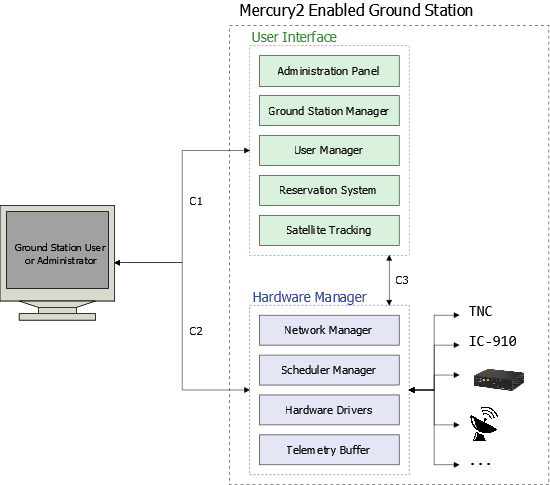
\includegraphics[scale=.55]{Architecture_Diagram.png}
	\caption{Mercury2 Architecture Overview}
	\label{architecture_diagram}
\end{figure}

%=== User Interface ===%
\section{User Interface}
\label{sec:user_interface}
The user interface for Mercury2 will consist of an application running on a web server that will allow satellite and ground station operators to interact with the ground station. This web application will be responsible for managing user permissions, maintaining the ground station reservation schedule, providing ground station feedback to satellite operators during reservations, and sending commands to the hardware manager. Each major component of the user interface (illustrated in figure \ref{architecture_diagram}) will be described in further detail in the following sections.

\subparagraph{Platform Details}
The user interface application will be developed on top of a popular Python MVC web framework, known as \textit{Django}, running on an Apache web server. Django comes with many useful features right out of the box such as user management, user input sterilization, and a well developed templating system which will greatly reduce development time. The application will make use of a MySQL database to store user information, schedule details, and user activity logs, among other things.

\subparagraph{Security}
Because the user interface has access to sensitive user information and direct control over the ground station, security and access control will be very important. Fortunately, Django comes with many useful security features by default such as user input sterilization, protection against cross-site scripting attacks, password hashing, and user permission management. User permissions will be configured to give users various levels of control over the ground station depending on their role (satellite operator, ground station operator, administrator, etc.). This mechanism will be detailed in the User Manager section (\ref{sec:user_permissions}). In addition, the security protocols used to protect the hardware manager data and command streams will be covered in section \ref{sec:data_flow}.

\subsection{User Manager}
\label{sec:user_manager}
The user management section of the user interface is responsible for maintaining user accounts and permissions across the whole Mercury2 system. It will provide several standard user features such as registration, logging in, and password recovery. Administrators will be able to set user registrations to either be open (anybody can create an account) or closed (an administrator or ground station operator needs to approve each account). Once a user has created an account, administrators will be able to give them various permissions which will determine what they can do on the website. This, and several other user manager features, are described in the sections below.

\subsubsection{User Roles and Permissions}
\label{sec:user_permissions}
The user permission system will manage the permissions that determine what any given user can do on the website. Most actions in the user interface will have an associated permission that can be set. The ground station administrator will be able to create permission groups that define the permissions for an arbitrary group of users. For example, an administrator could create a "users" group that contains the permissions for creating a new reservation and for creating a new user group (explained in the next section) that would be applied to new users by default. Permission groups will also be able to inherit permissions from other groups. The following table lists several possible permission groups that could be used.

\begin{table}[H]
\begin{center}
{\renewcommand{\arraystretch}{1.5}
\begin{tabular}{p{2in}|p{1in}|p{3in}}
	\bf Permission Group & \bf Inherits From & \bf Possible Permissions \\ 
	\hline
		Administrators 
	&
		All
	&
		\textbullet~ Given to the user that sets up the website \par
		\textbullet~ All possible permissions \par
		\textbullet~ Change permission groups \par
		\textbullet~ Create other administrators \par
		\textbullet~ Manage hardware pipelines
	\\ \hline
		Ground Station Operators
	&
		Users
	&
		\textbullet~ Approve or deny reservation requests \par
		\textbullet~ Modify reservation schedule \par
		\textbullet~ Create or modify user accounts \par
		\textbullet~ Assume manual control of the ground station \par
		\textbullet~ View any active satellite tracking panel (used to view ground station data streams during reservations) \par
		\textbullet~ View complete ground station status report
	\\ \hline
		Users
	&
		None
	&
		\textbullet~ Create pipeline reservations \par
		\textbullet~ View own satellite tracking panels during reservations \par
		\textbullet~ Create and manage user groups (explained in the next section) \par
		\textbullet~ Modify own account \par
		\textbullet~ Access read only version of ground station schedule \par
		\textbullet~ Create ground station access keys (explained in the \textit{Security} section below)
	\\
\end{tabular}}
\end{center}
\end{table}

\subsubsection{User Groups}
\label{sec:user_groups}
Because the majority of satellites are operated by a team, users will be able to create custom user groups to share information with their team members. Users will be able to add members to their groups as they please. When creating reservations, users will have the option of making the reservation available to any of their groups. This will allow other group members to view the satellite tracking page when the reservation becomes active. Users will also be able to share their saved reservation preferences (e.g. tracking information, pipeline selection, hardware settings, etc.) with their group. Each group will receive a simple page containing a group member list, a history of prior reservations, and a calendar containing all of the group's upcoming reservations.

\subsubsection{Security}
\label{sec:user_security}
As user security is very important for Mercury2, all user passwords will be salted and hashed before being stored in the database. To ensure that only the correct user can control the ground station during their reservation, a key based authentication system will be used (HMAC-SHA256). The account management panel will contain a section for creating and deleting ground station access keys. When a user creates a reservation they will be able to select which key pair they want to use for the connection. Whenever the user attempts to connect to the hardware manager, it will send the keys to the user interface for validation. Data stream encryption is explained in greater detail in section \ref{sec:connection_c2}.

\subparagraph{Logging}
Every action that any user performs in the user interface will be logged to a collection of log files. The administration panel will include a small utility for browsing these logs. 

\subsection{Reservation System}
\label{sec:reservations}
Mercury2 will include a reservation management system that will be used to coordinate access to the the ground station. Reservations are made for collections of dependent hardware called pipelines. A hardware pipeline is simply the set of hardware items that is required to perform a given task (e.g. transmit or receive from the radio). Once a pipeline has been reserved, no other pipelines that use any of the hardware items from the first pipeline can be reserved for the same period. See \ref{sec:hardware_manager} for more on hardware pipelines.

Once a user has created an account, they will be able reserve hardware pipelines. On the reservation page the satellite operator would first specify which available hardware pipeline they would like to reserve. Next, they will select a date, time, and duration for their pass either manually or by selecting a pass from the provided list of upcoming passes. Finally, if the requested time slot was available, the satellite operator will be able to pre-enter the configuration settings for each piece of hardware in the pipeline. The reservation will then be added to the ground station's reservation schedule. Ground station administrators can optionally require that any new reservations be approved before being added to the schedule. The new reservation will be sent to the appropriate hardware manager the next time the hardware manager synchronizes its schedule. An example of the scheduling flow is included in \ref{schedule_flow}.

\subparagraph{Priority Access} When creating reservations, users will also be able to specify a priority for the reservation. If the user needs immediate emergency access to the ground station and there is a time conflict with another reservation, they can set the priority to "urgent" which will notify the ground station operator who can then approve or deny the override.

\subsubsection{Shared Reservations}
Users can optionally share their reservations with any groups that they are a member of. If a reservation is shared with a group, anyone in that group will be able to access the reservation's tracking page when the reservation starts (however only one user may connect to or control the ground station at any given time). In addition, the reservation's parameters become available as defaults for everyone in the group allowing for quick rescheduling of common events.

\subsubsection{Reservation Schedule}
The user interface component of Mercury2 maintains the master schedule for the ground station. The master schedule is composed of all of the user reservations and scheduling time restrictions. Every time a user attempts to create a reservation, this master schedule is consulted to make sure the time slot is free. Periodically, the configured hardware managers will synchronize their schedules with master schedule. As mentioned above, ground station administrators or operators will be able to block out any periods of time in the schedule. For example, a ground station operator might chose to disallow access to the ground station every evening for an hour to perform maintenance. Subsets of the reservation schedule will be displayed on various pages such as the main reservation  and group pages.
 
\subsubsection{Hazardous Weather Detection}
This feature will safe guard the ground station from hazardous weather such as thunderstorms, snow storms, and heavy rain. Using the ground station's location and online weather APIs, Mercury2 will periodically check for hazardous weather. If it is detected, the ground station will be locked down and any existing reservations for the period will be canceled. 

\subsection{Satellite Tracking Panel}
\label{sec:tracking_panel}
Every reservation created has an associated tracking page. When a user visits this page before the reservation begins, it contains information about the reservation as well as the ground station connection settings (IP address, port, which key to use, etc.). In addition, a retroTrack style tracker with a Az/El chart will be displayed if a TLE was specified in the reservation. Once the reservation begins additional data streams from the ground station will become available, primarily the status of each of the active pipeline's hardware devices. Many other data streams are possible such as web cam feeds and signal strength waterfall plots. What data streams are available will depend on the ground station configuration and available bandwidth.

Satellite operators will also be able to command the ground station from the satellite tracking page. Each controllable hardware device in the pipeline will have an associated command form in the user interface that will be displayed on the tracking page. When the user commands a hardware device, the command will be sent to the hardware manager via an AJAX request. Although multiple users can view the tracking page at once, only one user will be able to submit commands from it.

\subsection{Ground Station Manager}
\label{sec:ground_station_manager}
The ground station management section of the user interface will allow users to view the complete health of each hardware manager as reported in the hardware manager's last health update. Users with the appropriate permissions (i.e. administrators or ground station operators) will also be able to send commands directly to the hardware manager from this interface. However, they will only be allowed to do this if no other users are currently commanding the ground station (whose reservations they can cancel, if need be). This panel will also contain a display of the main schedule and a link to the tracking page of the currently active reservation (if any). If there are any pending reservations or override requests, they will be be displayed here for the ground station operators to act on.

\subsection{Administration Panel}
\label{sec:admin_panel}
The user interface will include an administration panel to configure the website and ground station. This interface will only be available to users with the required permissions (administrators and possibly ground station operators). From the administration panel administrators will be able to manage user accounts, configure website settings, configure available hardware manager instances, modify permission settings and groups, and view application logs and statistics.

%=== Hardware Manager ===%
\section{Hardware Manager}
\label{sec:hardware_manager}
The hardware manager component of Mercury2 will consist of a relatively simple python application running on a computer physically attached to the ground station hardware. Its responsibilities will include synchronizing its reservation schedule with the user interface's, configuring hardware and network sockets when a reservation begins, and recording and transmitting satellite telemetry throughout the course of the reservation. Mercury2 will support multiple instances of the hardware manager running on separate computers. This is useful for decentralized ground stations. Each major component of the hardware manager (illustrated in figure \ref{architecture_diagram}) will be described in further detail in the following sections. 

\subparagraph{Hardware Pipelines}
One of the core concepts of the Mercury2 ground station system is that of a hardware pipeline. A hardware pipeline is simply a set of hardware devices, attached to the computer running an instance of the hardware manager, that are needed to perform a given task. The available hardware pipelines and their dependencies are defined by the ground station administrator when they first setup the hardware manager instance. Each hardware pipeline must also have specified "data in" and "data out" hardware devices which indicate where in the pipeline the user data stream should be fed into, and read out of. When a user creates a reservation in the user interface, they are reserving access a hardware pipeline. Multiple pipelines can be reserved for the same time slot, however only if they don't share any hardware devices.

\subparagraph{Twisted Framework}
The hardware manager will be built on top of an asynchronous event-driven Python framework known as \textit{Twisted}\footnote{For a comprehensive tutorial on Twisted see: http://krondo.com/blog/?page\_id=1327}. Twisted will be used because it will allow data to be passed from the network manager to the drivers (and vice versa) in asynchronous fashion with relative ease. Twisted represents all connections made with users or hardware devices as instances of a "protocol" class. These protocol classes asynchronously respond to events from the protocol (i.e. network or hardware device) as they arrive.

\begin{figure}[hbtp]
	\centering
	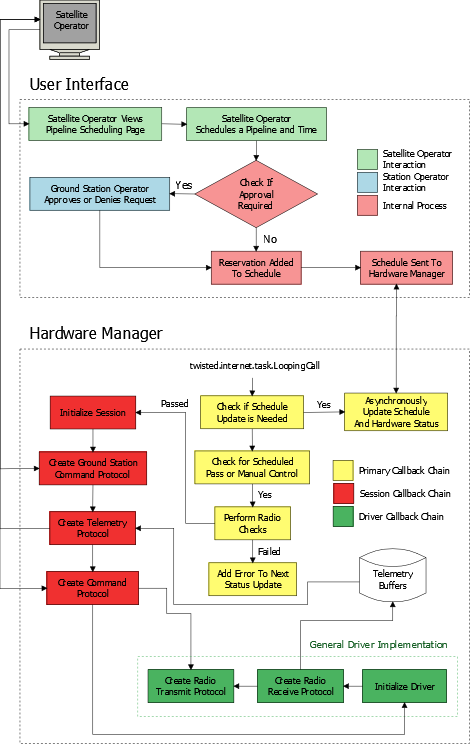
\includegraphics[scale=.55]{reservation_flow.png}
	\caption{Scheduling Flow Example}
	\label{schedule_flow}
\end{figure}

\subsection{Network Manager}
\label{sec:network_manager}
The network manager component of the hardware manager is responsible for providing the mechanisms to periodically update the hardware manager's reservation schedule, open command and data sockets for satellite and ground station operators, and report the hardware manager's state and health to the user interface. As stated above, Twisted programming methodologies will be used to create the network interface.  Each connection type that the network manager will make will be explained further in \ref{sec:data_flow}.

\subsection{Schedule Manager}
\label{sec:schedule_manager}
The schedule manager will be responsible for parsing and responding to changes in the schedule fetched from the user interface (via the network manager). It will consist of a main program loop (based on the \textit{twisted.internet.task.LoopingCall} class) that coordinates the various components of the hardware manager. The schedule manager can be said to "run" the hardware manager instance because it is responsible for running the other components of the application. Each of the scheduler manager's primary functions are described in the list below. In addition, an example reservation flow is illustrated in figure \ref{schedule_flow} that shows how the schedule manager (in yellow) interacts with the other components.

\begin{description}
	\item[Synchronize Reservation Schedule] Periodically, the schedule manager will instruct the network manager to download a new copy of the hardware manager's reservation schedule. The new schedule will then be parsed and merged in with local schedule.
	\item[Report Station Health \& State] The schedule manager will also occasionally serialize its state (most likely into JSON) and send it to the user interface (via the network manager). This state will include the parameters of each connected hardware device and of the hardware manager itself (e.g. currently executing task, buffer size, etc.). The user manager will display subsets of the state on various pages such as the ground station manager (section \ref{sec:ground_station_manager}) and satellite tracking pages (section \ref{sec:tracking_panel}).
	\item[Execute Reservations] When the schedule manager checks the schedule and determines that a reservation has begun, it will first create a new instance of the "session" class (which is used to represent each reservation). The session object will first verify that each hardware item in the reservation's pipeline is active and responding to commands. Next, it will configure each hardware item as per the schedule. Finally, the session object will create (Twisted) protocols for the ground station command and satellite command/telemetry streams, link them to the appropriate buffers, and update the application state.
	\item[Ending Running Reservations] Once the schedule manager determines that a reservation has ended, it will instruct the reservation's session object to destroy itself and the protocol objects that it created. However, this will only happen once all data from the reservation period has been transmitted to the ground station or satellite operator. Regardless of whether or not all of the data has been transmitted, the schedule manager will then unlock itself and update its state to indicate that it is ready to begin another reservation. The data transfer from the previous reservation will continue in the background until it is completed.
\end{description}

\subsubsection{Representing Ground Station State}
\label{sec:state}
The hardware manager's state will be maintained in a singleton class that gets initiated at run time. This class will contain the methods needed to read and update the following state items.

\begin{itemize}
	\item Local reservation schedule
	\item Currently executing task
	\item Hardware device parameters
	\item Ground station configuration (loaded at run time)
\end{itemize}

The state class will also provide a method to serialize the state (most likely into a JSON string) for periodic transmission to the user interface. The ground station configuration mentioned in the list above will stored in a YAML file and loaded at run time.

\subsection{Hardware Drivers}
\label{sec:drivers}
Each hardware device that is connected to the hardware manager will require its own driver class. The amount of functionality that this driver exposes is dependent on what the device supports and how developed the driver is. At the very least, each driver must be able to report the state of its associated hardware device (e.g. power on/off, frequency, etc.). In addition, many drivers will include methods to change the device configuration. Some drivers, such as radio drivers, must also provide the means to pass and receive data to and from the device. Because the hardware manager is asynchronous, it is important that the hardware drivers take steps avoid blocking the program execution.

Because the functionality of devices can vary so dramatically, each driver will be responsible for parsing ground station commands for that device. When the hardware manager receives a ground station command, it will determine which hardware device it is addressed to and pass it to the that device's driver. The driver will then be responsible for executing the command and reporting the status back to the hardware manager. See section \ref{sec:connection_c2_commands} for more on this.

\subsection{Telemetry Buffer and Persistence}
\label{sec:telemetry_buffer}
All information transmitted from and received by the hardware manager will be recorded in a session specific telemetry buffer. This serves two purposes. First, it allows data streams to be buffered until they can be transmitted over the network. For example, if a radio is outputting data at a faster rate than the network can support, it will be stored in the buffer until it is transmitted to the satellite operator. Second, it enables the hardware manager to maintain copies of all of the data that gets passed through the hardware manager. This will allow ground station operators to recover data if the network connection was lost in the middle of a transmission, for example. Because the buffers can become very large, ground station administrators will be able to decide how often buffer files should be purged.

\subparagraph{How Protocols Use Buffers}
As mentioned in section \ref{sec:drivers}, each device or network interface will be associated with a Twisted protocol class. These classes will respond to events (e.g. "data received" or "connection opened") and act accordingly. Because network interfaces and devices are both represented using Twisted protocols, they will need some way to pass information to each other. This is done using buffers. As an example, consider the satellite data stream. When a user transmits some data to the hardware manager the listening network protocol will write that data to one of the session's buffer files. It will then pass the buffer file to the destination driver and inform it that there is new data to be read from the file. The driver's protocol will then read the data and pass it to the hardware device. Similar buffers will be used for each device/data stream.

%=== Data Flow ===%
\section{Data Flow}
\label{sec:data_flow}
A Mercury2 enabled ground station consists of three main entities: the user (satellite or ground station operator), the user interface (section \ref{sec:user_interface}), and the hardware manager (section \ref{sec:hardware_manager}). This section will explain the various data paths, protocols, and security measures used to move data between these entities. Each data path in figure \ref{architecture_diagram} will be covered in the following sections.

\subsection{C1: User Interface Interactions}
\label{sec:connection_c1}
The user will connect to the user interface using a standard SSL encrypted HTTP connection through their web browser. All data entered by the user (except for ground station commands and hardware pipeline connections) will pass through this connection. During a scheduled reservation, the user may submit ground station commands from their browser. This is done through connection C3 (section \ref{sec:connection_c3}).

\subsection{C2: Hardware Pipeline Connection and Ground Station Commands}
\label{sec:connection_c2}
This is the connection that the satellite or ground station operator will use to command the ground station and connect to the hardware pipeline during their reservation.

\subsubsection{Ground Station Commands}
\label{sec:connection_c2_commands}
When the hardware manager is first started, it will open a ground station command socket that users will use to submit commands to the hardware manager. A key based authentication system (HMAC-SHA256) will be used to encrypt this connection using the key for the user specified in the schedule (see section \ref{sec:user_security} for how the user generates the keys). When a connection is made, the hardware manager will send the key to the user interface (via connection C3) for authentication. Multiple users may command the ground station at the same time. However, normal users will only be able to execute a few commands unless they have an active reservation. A few read-only commands, such as reporting the current ground station time, can be made at any time. In addition, other users may not submit commands that would interfere with the current reservation. This includes administrators and ground station operators. If they want to take manual control of the ground station without a reservation, they must switch it to manual mode in the user interface. During a reservation, a user may submit commands to the ground station using the tracking interface (section \ref{sec:tracking_panel}). The user interface builds the command for the the user and sends it with the user's key using the process explained above.

\paragraph{Ground Station Command Language}
Commands will be sent to the hardware manager using a ground station command language. This language will consist of JSON structures containing the user key and meta data about the command. When a command is received, the user key is first validated. If the user key is valid, the command is then parsed and redirected to the appropriate component or driver. The driver then executes the command and returns the result.

\subsubsection{Hardware Pipeline Connection}
During a reservation, users will be able to use this connection to send and receive data directly to the hardware pipeline. As explained in section \ref{sec:hardware_manager}, hardware pipelines have defined "data in" or "data out" devices. When a user submits data to the pipeline, it will be fed to the "data in" device. Likewise, when the "data out" device generates data it will be transmitted to the user over this socket. Like the ground station command socket, this connection will be encrypted using the same key based encryption system described in the previous section. Multiple users may be connected to the same hardware pipeline, but only one may send data during any given period (i.e. the reservation period). However, if a reservation ends without all of the data being transmitted back to the user the connection will be maintained in a read-only mode until the data buffer has been completely transmitted.

\subsection{C3: Schedule Updates, Health Reports, and Key Validations}
\label{sec:connection_c3}
This connection will consist of a SSL encrypted HTTP connection that the hardware manager will use for several maintenance operations. The primary function of this connection will be to maintain the ground station state. Periodically (a few times a minute), the hardware manager will package its state (section \ref{sec:state}) into a JSON structure. It will then transmit this state to the user interface which will store it in its database. The user interface will respond with the latest version of the hardware manager's schedule. In addition, the hardware manager will use this connection to submit user connection keys to the user interface for authentication. 

% End the document
\end{document}
